% Euclidean Handout Number eight
\documentclass{tufte-handout}

%\geometry{showframe}% for debugging purposes -- displays the margins

%%%% Packages to make things pretty
\usepackage{amsmath,amsthm}
\usepackage{booktabs}
\usepackage{graphicx}
\setkeys{Gin}{width=\linewidth,totalheight=\textheight,keepaspectratio}
\graphicspath{{graphics/}}
\usepackage{units}
\usepackage{fancyvrb}
\fvset{fontsize=\normalsize}
\usepackage{multicol}
\usepackage{pdfpages}

%%%% Theorem Environments
\theoremstyle{definition}
\swapnumbers
\newtheorem{problem}{Problem}[section]
\newtheorem{conjecture}[problem]{Conjecture}
\newtheorem*{definition}{Definition}
\newtheorem*{theorem}{Theorem}
\newtheorem{question}[problem]{Question}
\newtheorem{challenge}[problem]{Challenge}
\newtheorem*{postulate}{Postulate}

%%%%%

\title{Euclidean Geometry:\\An Introduction to Mathematical Work}
\author[]{Math 3600}
\date{Fall 2020}

\begin{document}

\maketitle

\begin{marginfigure}
    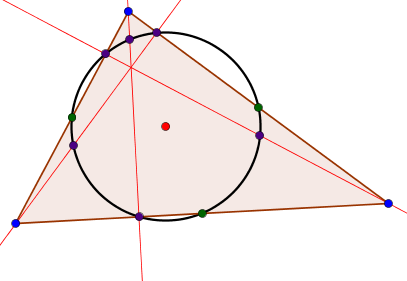
\includegraphics{NPC}
\end{marginfigure}

\setcounter{section}{8}
\section{The Center of a Triangle}

What might be called the center of a triangle? There have been many proposed answers to this question over the centuries. In this assignment, we study two of them.

\begin{conjecture}\label{conj:angle-bisectors-concurrent}
Let $ABC$ be a triangle, with rays $r$ and $s$ the angle bisectors at $A$ and $B$, respectively. Suppose that $r$ and $s$ meet at the point $I$ which lies inside the triangle. Draw lines $l$ and $m$ through $I$ that are perpendicular to $AC$ and $BC$ respectively. If $l$ meets $AC$ at point $X$ and $m$ meets $BC$ at $Y$, then triangle $IXC$ is congruent to triangle $IYC$.
\end{conjecture}


\begin{definition}\label{defn:concurrent}
Three segments (or lines or rays) are called \emph{concurrent} if they all pass through a common point.
\end{definition}

\begin{conjecture}\label{conj:incenter-concurrent}
The three angle bisectors of a triangle are concurrent.
\end{conjecture}

\begin{definition}\label{defn:incenter}
The point just discovered is called the \emph{incenter} of the triangle.
\end{definition}

\begin{conjecture}\label{conj:meeting-perp-bisectors}
Let $T$ be a triangle. For any pair of sides of $T$, the perpendicular bisectors of those sides meet. (That is, they are not parallel.)
\end{conjecture}

\begin{conjecture}\label{conj:circumcenter}
The three perpendicular bisectors of any triangle are concurrent.
\end{conjecture}

\begin{definition}\label{defn:circumcenter}
The point where the three perpendicular bisectors of a triangle meet is called the \emph{circumcenter} of the triangle.
\end{definition}








\vfill
\end{document}
